\documentclass[a4paper,10pt,twocolumn]{article}
\usepackage{amsmath}
\usepackage{amsfonts}
\usepackage{multicol}
\usepackage{{graphicx}}
\usepackage[margin=0.3in]{geometry}

\setlength\parindent{0pt}

\begin{document}
\textbf{16. PCA}\\
PCA diagonalize $p\times p$ corr coefficient matrix $r_{ij}=\sigma_{ij}/\sigma_i\sigma_j$. 

\textbf{18. Descriptive statistics}\\
Box-and-Whisker plot: \\
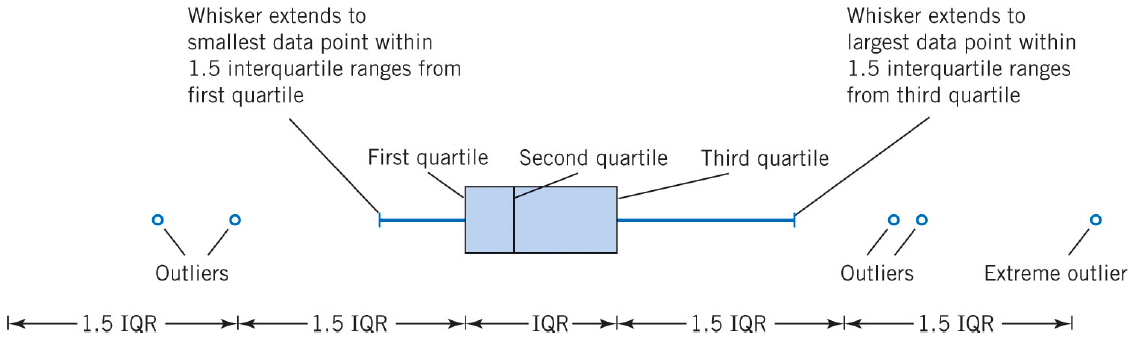
\includegraphics[width=0.8\columnwidth]{IQR.png}

Probability plot: $x_j(j-0.5)/n/CDF(x_j)$

\textbf{19. Sample mean and variance}\\
sample \textbf{mean}: $E(\bar{X})=\mu$\\
sample \textbf{variance}: $V(\bar{X})=\sigma^2/n$ \\
sample \textbf{std/standard error (SE)}: $\sigma/\sqrt{n}$

\textbf{central limit theorem}: the limiting form of the distribution of large n is the standard normal distribution: $Z=(\bar{X}-\mu)/(\sigma/\sqrt{n})$

Two popluations: the sampling distribution of $\bar{X}_1-\bar{X}_2$ with mean $\mu_{\bar{X}_1-\bar{X}_2}=\mu_1-\mu_2$ and variance $\sigma^2_{\bar{X}_1-\bar{X}_2}=\sigma_1^2/n_1+\sigma_2^2/n_2$ 

Sampling distribution of a \textbf{difference} in sample means: $Z=((\bar{X}_1-\bar{X}_2)-(\mu_1-\mu_2))/\sqrt{\sigma_1^2/n_1+\sigma_2^2/n_2}$

\textbf{20. point estimator}\\
Unbiased point estimator: $E(\hat{\Theta})=\Theta$\\
Bias: $E(\hat{\Theta})-\Theta$\\
\textbf{Mean Squared Error}: $MSE(\hat{\Theta})=E(\hat{\Theta}-\Theta)^2=V(\hat{\Theta})+bias^2$

\textbf{Methods of moment}: kth moment of random variable is $E(X^k)$.\\
First moment: $\mu=\int xf(x)dx$; second moment: $\mu^2+\sigma^2=\int x^2f(x)dx \rightarrow E(X^2)=Var(X)+E(X)^2$.

Moment estimators: $X_1,..,X_n$ with m unknown parameters. They are found by \textbf{equating first m population moments to first m sample moments}.

To estimate exponential distribution, 1st moment, $E(X)=\bar{x}=1/\lambda$; higher moment, $E(X^p)=p!/\lambda^p$

\textbf{Maximum likelihood}: $L(\theta)=f(x_1, \theta).f(x_2, \theta)...f(x_n,\theta)$. Maximum likelihood estimator (MLE) of $\theta$ is the value of $\theta$ that maximize $L(\theta)$. Use logarithm: $I(\theta)=ln L(\theta)$

\textbf{Exponential MLE}: $dlnL(\lambda)/d\lambda=n/\lambda-\sum x_i=0\rightarrow \lambda=n/\sum x_i=1/\bar{X}$

\textbf{Bernoulli MLE}: $\hat{p}=\sum x_i/n$

\textbf{Normal MLE for $\mu$}: $dln L(\mu)/d\mu=\sum(x_i-\mu)/\sigma^2=0\rightarrow \hat{\mu}=\bar{X}$

\textbf{MLE for poisson distribution}: $dln f(x_1,..,x_n|\lambda)/d\lambda=-n+\sum x_i/\lambda=0\rightarrow \lambda=\sum x_i/n$

\textbf{Sample variance}: $s^2=\sum (x_i-\bar(x))^2/(n-1)$. If mean $\mu$ is known, use n. $s^2=\sum (x_i-\mu)^2/n$

\textbf{21. Confidence intervals}: \\
two-sided: $Prob(L<\mu<R)=1-\alpha\rightarrow P(\bar{X}-Z_{\alpha/2}\sigma/\sqrt{n}<\mu<\bar{X}+Z_{\alpha/2}\sigma/\sqrt{n})=1-\alpha$; \\
one-sided: $Prob(\mu>R)=\alpha\rightarrow P(\bar{X}-\mu/\sigma\sqrt{n}<Z_\alpha)\rightarrow\mu>\bar{X}-Z_\alpha\sigma/\sqrt{n}$

\textbf{If sample is small and population variance is not known}, use sample variance $s^2=\sum (x_i-\bar{x})^2/n-1$ and use t-distribution instead of normal distribution.

t-distribution: $f(t)=(1+\cfrac{t^2}{n-1})^{-n/2}$, n is dof. 

Then the t confidence interval on $\mu$ is $\bar{x}-t_{\alpha/2,n-1}s/\sqrt{n}<\mu<\bar{x}+t_{\alpha/2,n-1}s/\sqrt{n}$

Confidence interval on the variance: $\cfrac{(n-1)s^2}{\chi^2_{\alpha/2,n-1}}<\sigma^2<\cfrac{(n-1)s^2}{\chi^2_{1-\alpha/2,n-1}}$

Large sample confidence interval for a population propotion: $\hat{p}-z_{\alpha/2}\sqrt{\cfrac{\hat{p}(1-\hat{p})}{n}} \le p \le \hat{p}+z_{\alpha/2}\sqrt{\cfrac{\hat{p}(1-\hat{p})}{n}}$

\textbf{22. Hypothesis Test}\\
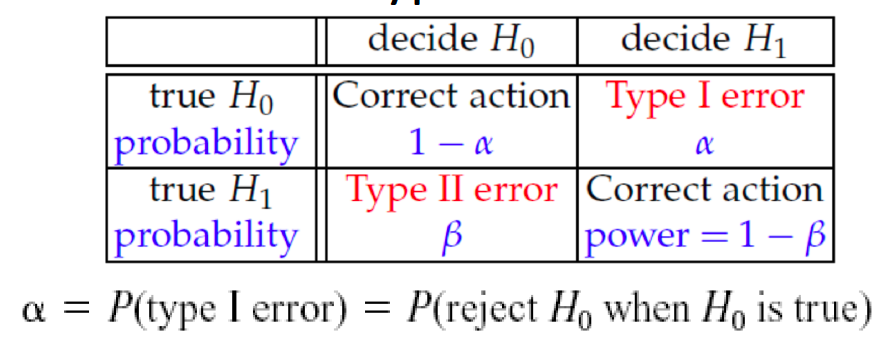
\includegraphics[width=0.8\columnwidth]{two_type_error.png}

If $H_1$ is \textbf{two-sided} hypothesis, P-value is $2(1-\Phi(|Z|))$, where $Z=(\bar(X)-\mu_0)/(s/\sqrt{n})$. If $\alpha$ is given, bounds are $\mu_0\mp z_{\alpha/2}*s$ to reject null hypothesis.

For \textbf{one-sided} $\mu_1>\mu_0$, it's $1-\Phi(Z)$; for $\mu_1<\mu_0$, it's $\Phi(Z)$. 

If sample size n is small, use t-distribution with n-1 DOF for two-sided P-value: $2(1-CDF_{Tdist}(|T|))$ where $T=\bar{X}-\mu_0/s\sqrt{n}$. Use $\mu_0\mp t_{\alpha/2,n-1}T$ to \textbf{reject null hypothesis}.

Type II error and choice of \textbf{sample size}, $n={z_{\alpha/2}+z_\beta}^2\sigma^2/\delta^2$, where $\delta=\mu-\mu_0$

m independent null hypothesis, at least one is false at significant threshold $\alpha_1$: Family-Wise Error Rate=$1-(1-\alpha_1)^m$; to get FWER < $\alpha$, $\alpha_1=\alpha/m$

Hypothesis test for a \textbf{difference} in means:\\
$H_0:\mu_1-\mu_2=\Delta_0=0$, test statistic: $Z_0=\cfrac{\bar{X_1}-\bar{X_2}-\Delta_0}{\sqrt{\sigma_1^2/n_1+\sigma_2^2/n_2}}$\\
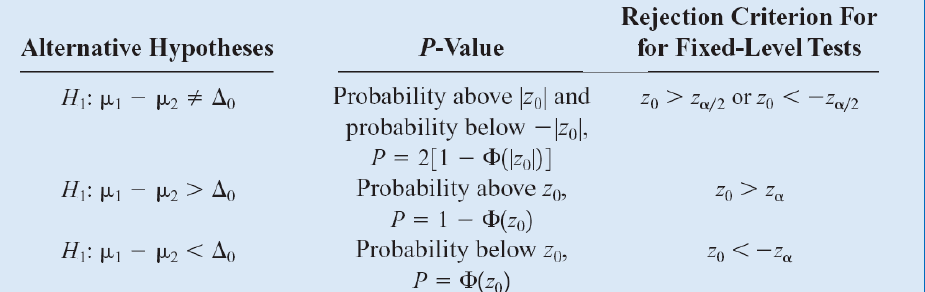
\includegraphics[width=0.8\columnwidth]{alternative_hyp.png}

If $\sigma_1^2\ne \sigma_2^2$, t-distribution with \textbf{DOF} $v=n_1+n_2-2$

\textbf{23. Goodness of fit test}
\textbf{Pearson $chi^2$ goodness of fit test}: $\chi_0^2=\sum_{i=1}^k(O_i-E_i)^2/E_i$, where $O_i$ is observed number and $E_i$ is expected number. P-value=P($H_0$ is correct)= $1-CDF_{chi-squared}(\chi_0^2, k-1)$.

How to test hypothesis if samples are drawn from same population: $P(group1;color=green)=P(group1)P(color=green)$.

$E_{green}(group1)=n_{tot}(group1/n_{tot})(green/n_{tot})$. And $\chi^2=\sum_{groups\&colors}^{n_{tot}}(O_{color}(group)-E_{color}(group))^2/E_{color}(group)$, where DOF is (colors-1)(groups-1)

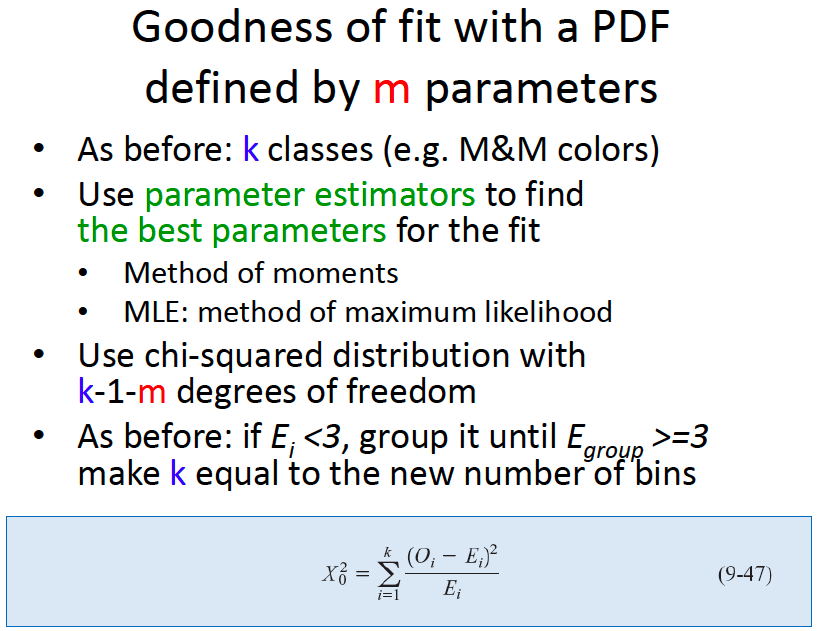
\includegraphics[width=0.8\columnwidth]{goodness_of_fit.png}

\textbf{Confidence interval for population variance}: $\chi_{n-1}^2=(n-1)S^2/\sigma^2$. 

Interval form: $\cfrac{(n-1)S^2}{\chi_{\alpha/2,n-1}^2}<\sigma^2<\cfrac{(n-1)S^2}{\chi_{1-\alpha/2,n-1}^2}$

\textbf{24. Regression analysis}\\
$Y=\beta_0+\beta_1X+\epsilon$, $\beta_1=Cov(X,Y)/Var(X);\beta_0=E(Y)-\beta_1E(X)$

Use least squares to estimate: $\beta_1=\cfrac{\sum y_ix_i-(\sum y_i)(\sum x_i)/n}{\sum x_i^2-(\sum x_i)^2/n}$

analysis of variance $\sum(y_i-\bar{y})^2=\sum(\hat{y_i}-\bar{y})^2+\sum(y_i-\hat{y_i})^2\rightarrow SS_T=SS_R+SS_E$

coefficient of determination: $R^2=SS_R/SS_T=1-SS_E/SS_T$

Estimate $\sigma_e^2$: $SS_E=\sum e_i^2=(n-2)\sigma_e^2$

Slope property: $E(\hat{\beta_1})=\beta_1; V(\hat{\beta_1})=\sigma^2/S_{xx}=\hat{\sigma_e^2}/n\sigma_x^2$

Intercept property: $E(\hat{\beta_0})=\beta_0; V(\hat{\beta_0})=\sigma^2[1/n+\bar{x}^2/S_{xx}]=\sigma_e^2[1+\mu_x^2/\sigma_x^2]/n$

\textbf{Hypothesis test}: H0: $\beta_1=0$; H1: $\beta_1\neq 0$

Use Z-test for large n: $Z=\hat{\beta_1}/(\hat{\sigma_e}/\sigma_x\sqrt{n})$. Reject H0 if $|Z|>Z_{\alpha/2}$

Use t-test for smaller n: $Z=\hat{\beta_1}/(\hat{\sigma_e}/\sigma_x\sqrt{n})$. Reject H0 if $|Z|>t_{\alpha/2,n-2}$
 
\textbf{25. Multiple linear regression}\\
$\mathbf{y=X\beta+\epsilon}$, where least square is $L=\sum e_i^2=(y-X\beta)'(y-X\beta)$. $dL/d\beta=0\rightarrow \hat{\beta}=(X'X)^{-1}X'y$

Property: $E(\hat{\beta})=\beta$, Covariance Matrix: $C=(X'X)^{-1}$; $V(\hat{\beta_j})=\sigma_e^2C_{jj}; cov(\hat{\beta_i},\hat{\beta_j})=\sigma_e^2C_{ij}$

Estimate $\sigma_e^2$, $\hat{\sigma_e^2}=SS_E/n-p$, where $p=k+1$

$R^2=1-SS_E/SS_T$; adjusted R-square: $R_{adj}^2=1-\cfrac{SS_E/(n-p)}{SS_T/(n-1)}$

\textbf{26. Clustering algorithm}\\
Hierarchical: agglomerative (eg, UPGMA), divisive

Non-hierarchical: PCA, K-means\\
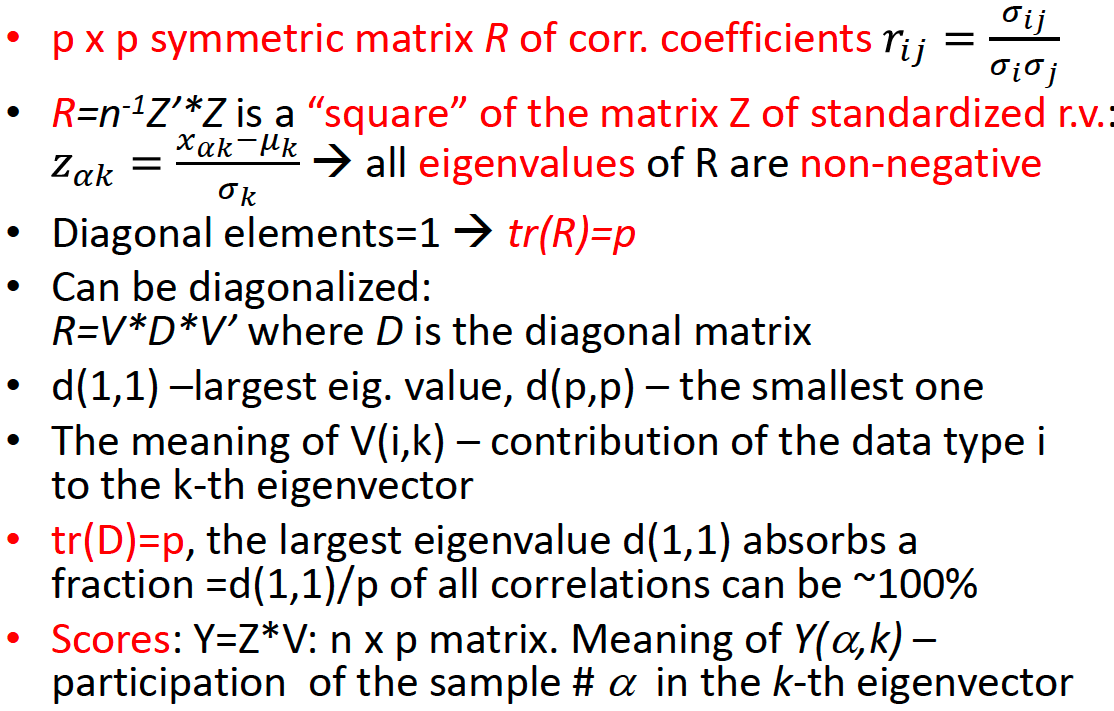
\includegraphics[width=0.8\columnwidth]{pca.png}

Distances: Euclidean:$\sqrt{\sum_i(x_i-y_i)^2}$; city block (Manhattan): $\sum_i|x_i-y_i|$; Canberra: $\sum(\cfrac{x_i-y_i}{x_i+y_i})$; correlation coefficient: $1-\rho(x,y)=1-\cfrac{Cov(x,y)}{\sqrt{Var(x).Var(y)}}$
\end{document}